\documentclass[11pt, twocolumn, twoside]{article}

\usepackage{graphicx}
\usepackage{amsmath, amssymb}
\usepackage{enumerate}
\usepackage{titleps}
\usepackage[top=1.25in,bottom=1in,right=0.75in,left=0.75in]{geometry}
\usepackage[parfill]{parskip}
\usepackage{titling}
\usepackage{hyperref}

\graphicspath{ {../images/} }

\newpagestyle{ruled}
{\setfoot{}{\thepage}{} \footrule}
\pagestyle{ruled}


\setlength{\droptitle}{-4em}   % This is your set screw
\posttitle{\par\end{center}\vskip 0.5em}


\title{6.867 Final Project Writeup} % Please change this
\date{}
\author {Vickie Ye and Alexandr Wang}


\begin{document}
\maketitle


\begin{abstract}
In this project, we compared different methods for facial expression recognition.
\end{abstract}

\section{Introduction}

\subsection{PCA}

\subsection{Facial Landmark Detection}

\subsection{Convolutional Neural Networks}

Convolutional Neural Networks (CNNs) are a particularly type of artificial neural network that works particularly well for image data. The structure of CNNs exploits strong local correlation in the inputs. This is done by enforcing local connectivity between neurons of adjacent layers. The inputs of a hidden unit at a particular layer $n$ are some locally-connected subset of the units of the previous layer $n-1$, done in such a way that the input to layer $n$ represent some tile of the units of layer $n-1$, where all the tiles overlap.

In addition, CNNs utilize shared parameterizations (weight vector and bias) across layers. By constraining the same types of weights across layers, essentially replicating units across layers, allows for features to be detected regardless to their position in the initial input, making the network much more robust to real world image data. Additionally, by constraining multiple weights to be the same reduces the parameters to be learnt, increasing learning efficiency.

\section{Experimental Details}
The dataset we used was taken from a Kaggle facial expression dataset.

\subsection{Convolutional Neural Network}

For implementing our convolutional neural network, we used TensorFlow for the entire implementation, i.e. training, inference, and evaluation.

\begin{figure}
	\centering
	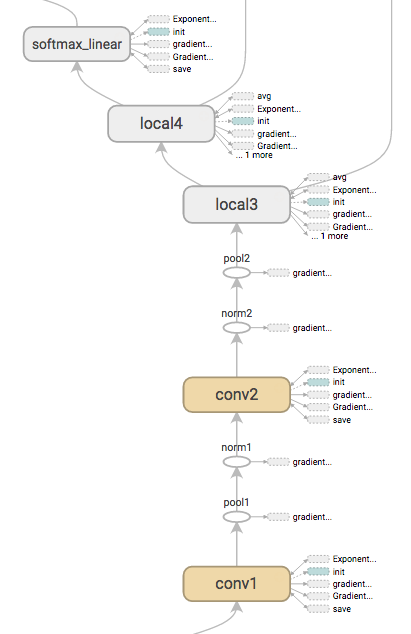
\includegraphics[width=3.25in]{inference_graph}
	\caption{TensorFlow computation graph for the neural network in the CNN we implemented, illustrating each of the layers.}
	\label{fig:inference}
\end{figure}

\section{Results and Analysis}

\begin{figure}
	\centering
	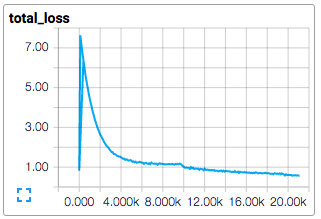
\includegraphics[width=3in]{total_loss}
	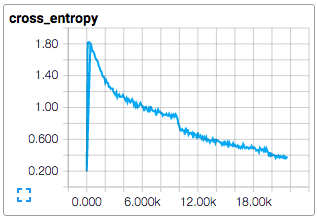
\includegraphics[width=3in]{cross_entropy}
	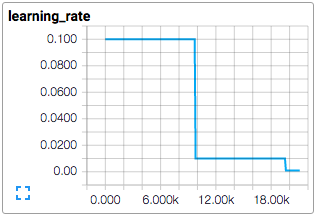
\includegraphics[width=3in]{learning_rate}
	\caption{The total loss, cross entropy, and learning rate of the convolutional neural net over time.}
	\label{fig:cnnloss}
\end{figure}

\begin{figure}
	\centering
	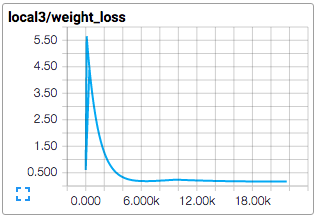
\includegraphics[width=3in]{local3_loss}
	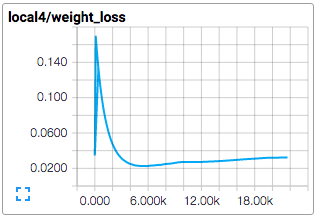
\includegraphics[width=3in]{local4_loss}
	\caption{The loss on the local3 layer and local4 layer over time in the convolutional neural net.}
	\label{fig:layer_loss}
\end{figure}


\begin{thebibliography}{9}
\bibitem{Lawrence}
Lawrence, S.; Giles, L.; Tsoi, A. C.; Back, A. D. (1997)
``Face Recognition: A Convolutional Neural-Network Approach"
\textit{Neural Networks, IEEE transactions on} 8 (1):98-113
\bibitem{Matsugu}
Matsugu, M.; Mori, K.; Mitari Y.; Kaneda Y. (2003)
``Subject independent facial expression recognition with robust face detection using a convolutional neural network"
\textit{Neural Networks} 16 (5):555-559
\end{thebibliography}

\end{document}
